\FloatBarrier
\section{Results}

\subsection{Model behaviour in the sandbox}
The frozen configuration was run once on all \NTest{} records of the PTB-XL test fold
(fold 10; Supplementary Table~\ref{tab:characteristics}). Every request returned a valid answer: no request failed, no
record needed the training-fold class prevalences reserved for failed records or a continuation after the API paused
a long tool loop, and no probability was out of range. The model ran code between \CodeRunsMin{} and \CodeRunsMax{}
times per record (mean \CodeRunsMean, median \CodeRunsMedian; Supplementary Fig.~\ref{fig:usage}a). The number
varied because, after each run, the model decided whether to run more code (see Section~\ref{sec:inference}): a record took several runs
when the model worked in steps, as in the example of Fig.~\ref{fig:example} described below, and more when a run ended
with an error. Per record, the model
produced a mean of \OutputTokensMean{} output tokens, including \ThinkingTokensMean{} reasoning tokens (Supplementary
Fig.~\ref{fig:usage}b); input tokens and cost are reported in Supplementary Section~\ref{app:cost} and Supplementary
Fig.~\ref{fig:usage}c. The \NBatches{} batches were sent one after another, and all results were obtained
\TestHours{} hours after the first was sent. A post hoc analysis of the transcripts showed that the model's code
filtered all \PHFilterFortyN{} records to a 0.5--40\,Hz band (\PHFilterSeparateN{} of them with separate high- and
low-pass filters) and used a peak detector in every record and a median function in \PHMedianN{} of them. The code
written for a record had a median of \PHSandboxLinesMedian{} non-empty lines (interquartile range
\PHSandboxLinesQOne--\PHSandboxLinesQThree). In the same analysis, \PHSandboxErrorsTotal{} of the
\PHSandboxCodeRunsTotal{} code runs (\PHSandboxErrorRatePct\%) ended with an error (a non-zero exit status or an
uncaught Python exception; see Section~\ref{sec:posthoc}). These errors occurred in \PHSandboxRecordsWithErrorN{} records. The model
recovered in \PHSandboxRecoveredN{} of them, whose last run succeeded; in the other \PHSandboxLastRunErrorN, the last run
failed after printing part of its output, and the model answered from that output and the output of earlier runs.

In a post hoc replay (see Section~\ref{sec:posthoc}), every code run was executed again offline on a local computer, and every run
reproduced its output. Of the \RPRuns{} runs, \RPIdentical{} (\RPIdenticalPct\%) printed byte-identical output and
\RPRounding{} the same output up to floating-point rounding (relative differences of at most \RPMaxRel). The other
\RPDifferent{} failed this strict comparison only trivially: two printed the indices of a sort (NumPy's default sort,
which is not stable) with tied values in a different order, one printed the name of the input directory, which the
API's sandbox chose at random, and two printed values close to zero at full precision, which differed by less than
$2\times10^{-12}$ (relative differences of up to $2.2\times10^{-9}$). All \RPErrorsReproduced{} errors recurred with the same exception type, and no other run failed. The printed
output on which the model based its answers can thus be reproduced without the API, from the released transcripts and
record files.

The model did not work the way the prompt asked (post hoc; Supplementary Table~\ref{tab:provenance}). The prompt
asked it to compute and print a complete measurement table before judging; printed output with labels for QRS, PR, QT
and axis together appeared in \PHFullTablePct\% of records. The printed output carried a label for heart rate in
\PHPrintedHrPct\% of records and for QRS in \PHPrintedQrsPct\%, and a per-lead table of R and S amplitudes in
\PHLeadAmplitudePct\%, but a label for the PR interval in only \PHPrintedPrPct\%, for QT or QTc in \PHPrintedQtcPct\%,
for the axis in \PHPrintedAxisPct\% and for a Sokolow--Lyon sum in \PHPrintedSokolowPct\%. For most of the PR
intervals, QT or QTc intervals and axes stated in the key findings (the answer's free-text field, which the prompt
limited to two sentences), no value was printed under the measurement's own label. In \PHDumpPct\% of records a code run
printed a line of 20 or more numbers, typically median-beat samples at reduced time resolution (records that printed
samples only on shorter lines are not counted). Among the records whose stated PR interval, QTc or axis had no
printed label, \PHDumpUnlabelledPrPct\%, \PHDumpUnlabelledQtcPct\% and \PHDumpUnlabelledAxisPct\%, respectively,
printed such lines. This suggests that the model read those intervals and axes from median-beat samples it printed,
as the record shown in Fig.~\ref{fig:example} illustrates for the PR interval: its reasoning summary, given with the
full transcript in Supplementary Section~\ref{app:transcript}, says that the PR interval was estimated from sample
positions. The label analysis itself cannot show where a stated value came from. The model thus used code mainly to build median beats from the filtered
recording, in leads, segments and resolution of its own choosing, and appears to have read numbers from them.

Figure~\ref{fig:example} shows one validation-fold record, read with the frozen prompt during development and
selected by the rule given in the legend. Unlike most test records, its code printed labelled QT and axis values
(a QT or QTc label was printed in \PHPrintedQtcPct\% and an axis label in \PHPrintedAxisPct\% of test records). The model received the raw recording as a file, with age and sex in the user message
(Fig.~\ref{fig:example}a), and used \ExampleCodeRuns{} code runs. In the first, it read the start of the file. In the
second (Fig.~\ref{fig:example}b), it band-pass filtered all leads, detected beats, formed a median beat per lead and
printed samples of it. In the third, it printed further samples to locate the QRS onset. In the fourth, it computed QRS
onset and offset (a QRS duration of \ExampleQRSPrinted\,ms), per-lead amplitudes and ST levels, QT and axis
(Fig.~\ref{fig:example}c). It answered that the record showed high precordial voltage without strain in a
\ExampleAge-year-old man, possibly a normal finding (Fig.~\ref{fig:example}e), and gave probabilities of
\ExamplePHYP{} for HYP and \ExamplePNORM{} for NORM (Fig.~\ref{fig:example}d); the record is labelled left
ventricular hypertrophy (LVH). The stated QRS duration was rounded from the printed one (about 100\,ms for
\ExampleQRSPrinted\,ms), but the stated axis differed from the printed one (near $+$\ExampleAxisStated$^\circ$ for a
printed value of about \ExampleAxisPrinted$^\circ$; the reasoning summary gives $+30^\circ$ to $+60^\circ$). Neither the
PR interval nor the Sokolow--Lyon sum was printed; the model added the Sokolow--Lyon sum from printed amplitudes. The user message and the
complete transcript are in Supplementary Sections~\ref{app:example} and~\ref{app:transcript}.

\begin{figure}[tbp]
  \centering
  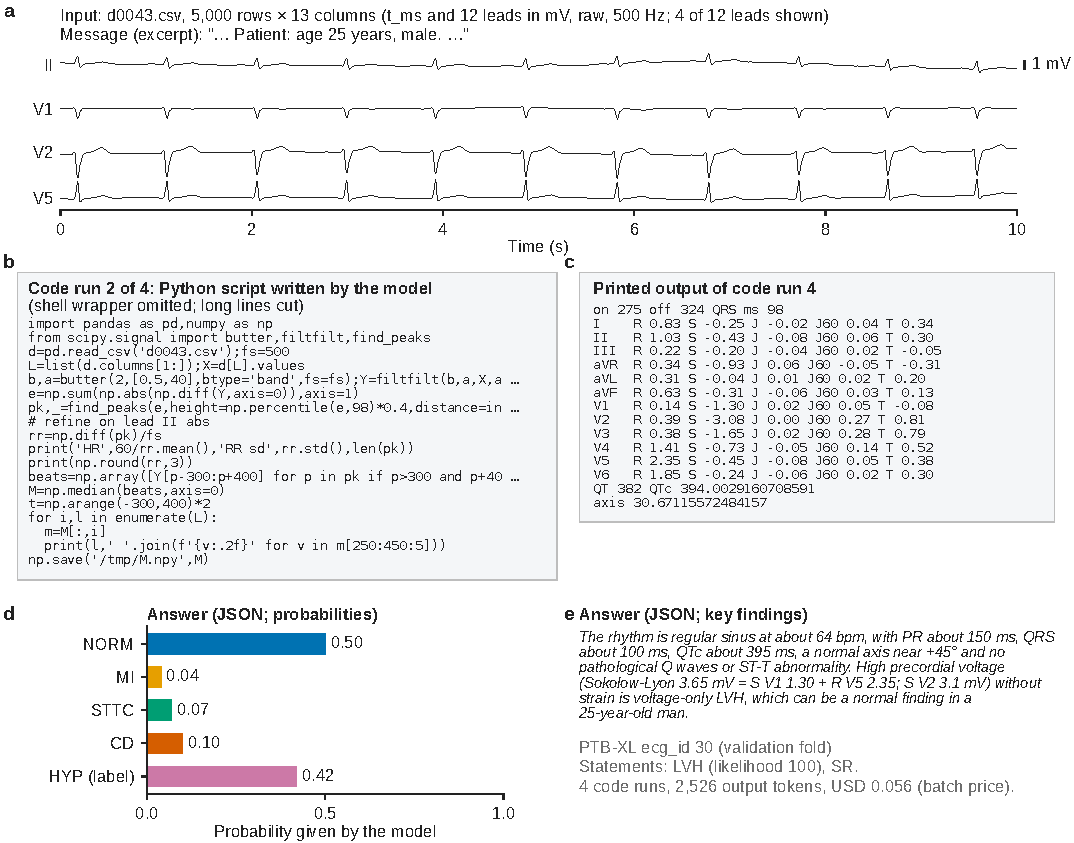
\includegraphics[width=\linewidth]{Figure_1}
  \caption{\textbf{One record from file to answer.} \textbf{a}, The input: a CSV file with the raw 10-second, 12-lead
  recording (4 of 12 leads shown; unfiltered, with baseline offsets as stored in PTB-XL), and the patient's age and sex, given
  in the user message (the complete message is in Supplementary Section~\ref{app:example}). \textbf{b}, The Python
  script of the second of \ExampleCodeRuns{} code runs, as written by the model, without its shell wrapper and with long
  lines cut (\ldots): a 0.5--40\,Hz band-pass filter, beat detection on a multi-lead envelope, RR intervals and a
  median beat per lead, whose samples it printed at 10-ms steps. \textbf{c}, The complete output of the last code run,
  as printed: QRS onset and offset (in samples) and duration (ms); per lead, R and S amplitudes, ST level at the J point
  (J) and 60\,ms later (J60) and T amplitude (mV); QT and Bazett-corrected QTc (ms) and frontal axis (degrees).
  \textbf{d}, \textbf{e}, The answer: five probabilities (``label'' marks the record's PTB-XL superclass) and the key
  findings, the answer's free-text field, which the prompt limited to two sentences. The grey note gives the record's
  PTB-XL statements (LVH, left ventricular hypertrophy; SR, sinus rhythm), code runs, output tokens and cost. The record
  (PTB-XL \texttt{ecg\_id} \ExampleECGID, validation fold) was chosen by a fixed rule, not by its result: the lowest
  \texttt{ecg\_id} whose only superclass is HYP among the validation records read with the frozen prompt. The complete
  transcript is in Supplementary Section~\ref{app:transcript}.}
  \label{fig:example}
\end{figure}

\subsection{Discrimination on the test fold}
Macro AUROC on the test fold, the primary endpoint, was \MainAUROC, with a 95\% confidence interval (CI) of
\MainAUROCLow--\MainAUROCHigh{} from \NBoot{} bootstrap resamples of the test records (see Section~\ref{sec:endpoints}), and macro average
precision (AUPRC) was \MainAUPRC. Per class, AUROC was \MainNORM{}
for NORM, \MainMI{} for MI, \MainSTTC{} for STTC, \MainCD{} for CD and \MainHYP{} for HYP (Fig.~\ref{fig:benchmark}b,
Supplementary Table~\ref{tab:perclass}; ROC and precision--recall curves in Supplementary Fig.~\ref{fig:curves}a,b).
Because the model also received the patient's age and sex, we compared it with an age-and-sex control: a logistic
regression per superclass that predicts the class from age and sex alone, fitted on the training folds (see Section~\ref{sec:endpoints}).
The control reached a macro AUROC of \AgeSexAUROC{} (Fig.~\ref{fig:benchmark}a). The model exceeded it by
$\CodeVsAgeSex$ (95\% CI $\CodeVsAgeSexLow$ to $\CodeVsAgeSexHigh$), and did so in every class (by $\CodeVsAgeSexNORM$
for NORM to $\CodeVsAgeSexHYP$ for HYP; Fig.~\ref{fig:benchmark}b). The \NTest{} test records come from
\PHNPatientsTest{} patients; \PHNPatientsMulti{} of them have two or more records, \PHNRecordsMulti{} records in
total, and records of the same patient are not independent. As a post hoc robustness check, we therefore repeated the
bootstrap on the same predictions, resampling patients with replacement, with each drawn patient contributing all of
their test records; the 95\% CI was nearly identical (\PHClusterLow--\PHClusterHigh).

Among published results on the PTB-XL superclass task (Fig.~\ref{fig:benchmark}a, Supplementary
Table~\ref{tab:benchmark}), the model's macro AUROC was \GapToBestPublishedAbs{} below the best result reported with
the same split, label definition and evaluation metric (\BestPublishedAUROC, reached by the ensemble of the original
benchmark models~\citep{Strodthoff2021} and by MultiresNet~\citep{shi2023multires}) and exceeded that of the best zero-shot
ECG--language model (\BestZeroShotAUROC~\citep{cai2025supreme}) by $\GapToBestZeroShot$. These comparisons are
informal: the published models' per-record predictions were not available, and their inputs differ (the original
benchmark models used 100\,Hz signals without age or sex).

\begin{figure}[tbp]
  \centering
  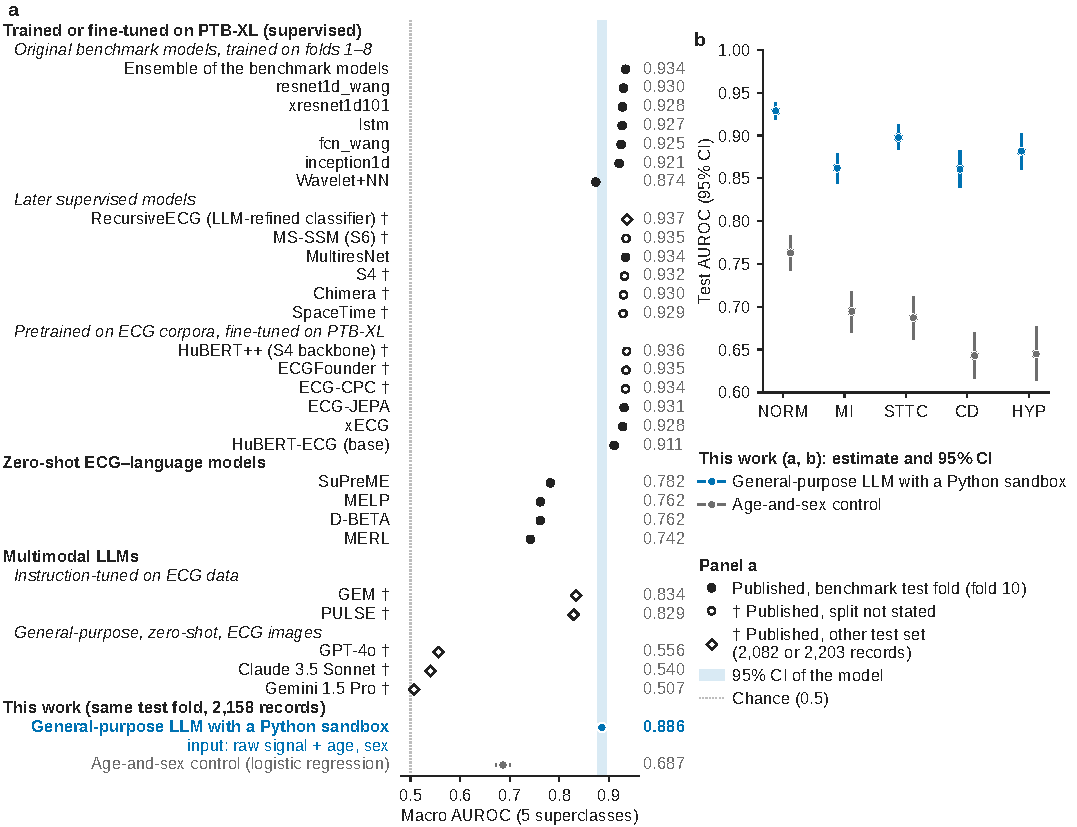
\includegraphics[width=\linewidth]{Figure_2}
  \caption{\textbf{Macro AUROC among published PTB-XL superclass results, and per class.} \textbf{a}, Published results
  as reported by their authors, grouped by model type and training (Supplementary Table~\ref{tab:benchmark} gives
  sources and inputs). Filled circles, results on the benchmark test fold (fold 10); $^\dagger$not directly
  comparable: split not stated (open circles), or a different test set (diamonds: RecursiveECG, a supervised model
  whose design an LLM agent revised, and the multimodal LLMs, including GEM~\citep{lan2025gem}). HuBERT-ECG's
  self-supervised pretraining corpus includes PTB-XL (unlabelled). This work: the LLM with a Python sandbox, which
  received the raw signal with age and sex, and the age-and-sex control, a logistic regression per class fitted on
  folds 1--8, both on all \NTest{} test-fold records with 95\% percentile bootstrap CIs (\NBoot{} resamples; the shaded
  band is the model's CI). \textbf{b}, Per-class AUROC of the model (blue) and the age-and-sex control (grey) on the
  test fold; bars are 95\% bootstrap CIs.}
  \label{fig:benchmark}
\end{figure}

\subsection{Discrimination by diagnostic statement}
We measured, post hoc, how well the model's superclass probability separated records with a given diagnostic
statement from records without that superclass (Fig.~\ref{fig:where}a, Supplementary Table~\ref{tab:statements}). This
was done for the \PHNStatements{} of PTB-XL's 44 diagnostic statements that had at least \PHMinStatement{} test
records. For example, for complete right bundle branch block, one of the statements under CD, we computed the AUROC of the model's
CD probability for the \PHStmtCRBBBN{} test records with that statement against all test records without CD. The model
gave only superclass probabilities, so this does not test whether the statement itself was identified. Separation was
best for complete right bundle branch block (AUROC \PHStmtCRBBB; \PHStmtCRBBBN{} records), complete left bundle branch
block (\PHStmtCLBBB; \PHStmtCLBBBN), left anterior fascicular block (\PHStmtLAFB; \PHStmtLAFBN), anterolateral
ischaemic change (\PHStmtISCAL; \PHStmtISCALN), anteroseptal infarction (\PHStmtASMI; \PHStmtASMIN) and non-specific
ischaemic change (\PHStmtISC; \PHStmtISCN). It was poorest for two statements defined by borderline QRS durations,
non-specific intraventricular conduction disturbance (\PHStmtIVCD; \PHStmtIVCDN) and incomplete right bundle branch
block (\PHStmtIRBBB; \PHStmtIRBBBN), and for left atrial overload (\PHStmtLAOLAE; \PHStmtLAOLAEN), inferior infarction
(\PHStmtIMI; \PHStmtIMIN) and lateral infarction (\PHStmtLMI; \PHStmtLMIN). Left ventricular hypertrophy reached
\PHStmtLVH{} (\PHStmtLVHN) and first-degree atrioventricular block \PHStmtOneAVB{} (\PHStmtOneAVBN); 95\% CIs are in
Supplementary Table~\ref{tab:statements}.

\begin{figure}[tbp]
  \centering
  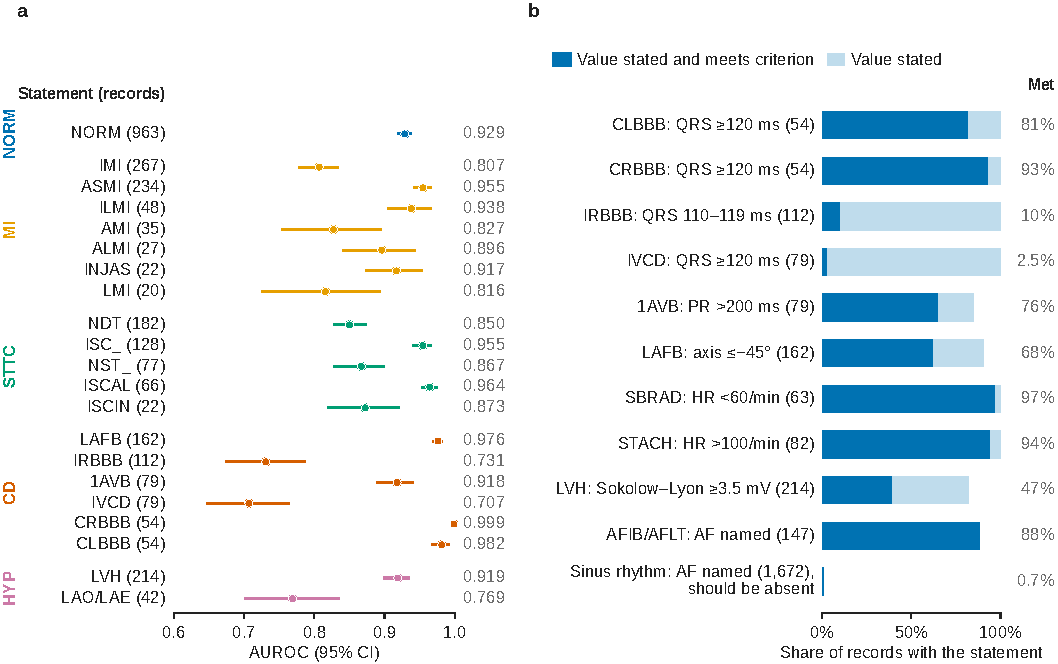
\includegraphics[width=\linewidth]{Figure_3}
  \caption{\textbf{Discrimination by diagnostic statement, and what the model stated (test fold, post hoc).}
  \textbf{a}, AUROC of the superclass probability for records with a diagnostic statement against records without that
  superclass, with 95\% stratified bootstrap CIs (\PHNStmtBoot{} resamples), for statements with at least
  \PHMinStatement{} test records, grouped by superclass (PTB-XL codes, defined below and in Supplementary
  Table~\ref{tab:statements}); number of records in brackets, AUROC at right. \textbf{b}, Measurements stated in the key
  findings of records with selected PTB-XL statements, against a criterion (number of records in brackets): light bars,
  share of all records with the statement whose key findings state the measurement; dark bars, share of all records
  with the statement whose stated value meets the criterion; at right (Met), the same share among the records that
  stated a value, as in the text and Supplementary Table~\ref{tab:measurements}. The criteria for QRS duration, PR
  interval and Sokolow--Lyon voltage are the frozen prompt's (for IVCD, QRS 120\,ms or more); the prompt gives no angle
  for fascicular block, so LAFB is shown against the AHA/ACCF/HRS criterion, an axis of $-45^\circ$ or more
  leftward~\citep{surawicz2009recommendations} ($-30^\circ$ or more in Supplementary Table~\ref{tab:measurements}).
  For the two rhythm rows (records with AFIB or AFLT, and records in sinus rhythm without them), the bar and Met give
  the share whose key findings name atrial fibrillation or flutter without negating it (AF named); in sinus rhythm, a
  short bar means agreement. Values were extracted from the text with regular expressions (Section~\ref{sec:posthoc}).
  IMI, ASMI, ILMI, AMI, ALMI, LMI: inferior, anteroseptal, inferolateral, anterior, anterolateral and lateral
  myocardial infarction; INJAS: subendocardial injury in anteroseptal leads; NDT: non-diagnostic T abnormalities;
  ISC\_, NST\_: non-specific ischaemic change and non-specific ST changes; ISCAL, ISCIN: ischaemic change in
  anterolateral and in inferior leads; CLBBB, CRBBB, IRBBB: complete left, complete right and incomplete right bundle
  branch block; IVCD: non-specific intraventricular conduction disturbance; 1AVB: first-degree atrioventricular block;
  LAFB: left anterior fascicular block; LVH: left ventricular hypertrophy; LAO/LAE: left atrial overload or
  enlargement; SBRAD, STACH: sinus bradycardia and tachycardia; HR: heart rate; AFIB, AFLT: atrial fibrillation and
  flutter.}
  \label{fig:where}
\end{figure}

\subsection{Stated measurements and the dataset's annotations}
The key findings stated a heart rate in \PHStatedCodeHr\% of test records, a QRS duration in
\PHStatedCodeQrs\%, an axis in \PHStatedCodeAxis\%, a PR interval in \PHStatedCodePr\%, a Sokolow--Lyon voltage in
\PHStatedCodeSokolow\% and a QTc in \PHStatedCodeQtc\% (post hoc; values extracted from the text with regular
expressions; see Section~\ref{sec:posthoc}). As described above, most of the stated PR intervals, QT or QTc intervals and axes appear to
have been read from printed samples rather than computed. We compared the stated values with the PTB-XL statements,
which were assigned or validated by cardiologists and are not measurements, so the comparison shows consistency, not accuracy
(Fig.~\ref{fig:where}b; the shares below are among records that stated the value, as in Supplementary
Table~\ref{tab:measurements}). Agreement was good for rate, rhythm and QRS duration in complete bundle branch block:
the stated rate was below 60/min in \PHMeasSBRADCodeCrit\% of records with sinus bradycardia and above 100/min in
\PHMeasSTACHCodeCrit\% of records with sinus tachycardia, and the stated QRS duration was 120\,ms or more in
\PHMeasCLBBBCodeCrit\% of records with complete left and \PHMeasCRBBBCodeCrit\% of records with complete right bundle
branch block. Rhythm is not part of the superclass task, but the key findings named atrial fibrillation or flutter in
\PHMeasAFCodeCrit\% of the \PHMeasAFN{} records with these rhythms and in \PHMeasSRAFCodeCrit\% of the \PHMeasSRAFN{}
records in sinus rhythm. Agreement was partial for the PR interval in first-degree atrioventricular block:
\PHMeasOneAVBCodeStated\% of these records stated one, and the stated PR exceeded 200\,ms in \PHMeasOneAVBCodeCrit\%
of those. It was also partial for the axis in left anterior fascicular block, which was $-45^\circ$ or more leftward
(the AHA/ACCF/HRS criterion~\citep{surawicz2009recommendations}) in \PHMeasLAFBFortyFiveCodeCrit\% and $-30^\circ$ or
more leftward in \PHMeasLAFBCodeCrit\%; the prompt gives no angle for fascicular block. In records labelled LVH, the
stated Sokolow--Lyon voltage met the prompt's criterion of 3.5\,mV in about half of those that stated one
(\PHMeasLVHCodeCrit\%; median \PHMeasLVHCodeMedian\,mV). Agreement was poor for incomplete right bundle branch block
(stated QRS duration 110--119\,ms in \PHMeasIRBBBCodeCrit\%) and for non-specific intraventricular conduction
disturbance (the prompt's criterion, 120\,ms or more, in \PHMeasIVCDCodeCrit\%); their median stated QRS durations
were \PHMeasIRBBBCodeMedian{} and \PHMeasIVCDCodeMedian\,ms, against \PHMeasNormQRSCodeMedian\,ms in records labelled
only NORM.

\subsection{Subgroups, calibration and the validation fold}
In post hoc subgroups (Supplementary Table~\ref{tab:subgroups}), macro AUROC was \PHSubWomen{} in
women and \PHSubMen{} in men, and \PHSubYoung{} under 50 years of age, \PHSubAgeMid{} at 50--69 years and \PHSubOld{} at
70 years or older. It was \PHSubAF{} in records with atrial fibrillation or flutter and \PHSubNotAF{} in other rhythms;
only \PHSubAFNormPos{} of the former were NORM, and the mean AUROC of the other four classes was \PHSubAFNoNorm{}
against \PHSubNotAFNoNorm. All age and rhythm strata were below the overall value (\MainAUROC); this is possible because the
overall AUROC also ranks records across strata, which differed steeply in class prevalence. Macro
AUROC was \PHSubNoise{} in records with a signal-quality flag in the PTB-XL metadata and
\PHSubNoNoise{} without, and it ranged from \PHSubDeviceMin{} to \PHSubDeviceMax{} across the \PHSubNDevices{} PTB-XL
device values with at least \PHMinSubgroup{} test records (\PHSubDeviceRecordsN{} of \NTest{} records), which are
confounded with recording sites. MI discrimination was lower when the annotator had assigned a lower likelihood to
the MI statement (post hoc; Supplementary Table~\ref{tab:subgroups}). With each MI-positive record grouped by the highest likelihood among its MI statements and
compared with all test records without MI, AUROC was \PHMILikHundred{} (\PHMILikHundredLow--\PHMILikHundredHigh) for
the \PHMILikHundredN{} records with likelihood 100, \PHMILikMid{} (\PHMILikMidLow--\PHMILikMidHigh) for the
\PHMILikMidN{} with 50--80 and \PHMILikLow{} (\PHMILikLowLow--\PHMILikLowHigh) for the \PHMILikLowN{} with 15--35;
the age-and-sex control reached \PHMILikHundredAgeSex, \PHMILikMidAgeSex{} and \PHMILikLowAgeSex{} in the same strata.
In a post hoc calibration analysis, which asks whether the probabilities can be read at face value (see Section~\ref{sec:posthoc};
Supplementary Fig.~\ref{fig:curves}c), calibration slopes of \PHSlopeMinNoCD--\PHSlopeMaxNoCD{} for NORM, MI, STTC and
HYP indicate probabilities that were not extreme enough. CD was close to calibrated, with a slope of \PHSlopeCD{} and an expected calibration error (ECE) of \PHECECD. MI was
underestimated in every probability bin above the lowest (overall mean probability \PHMeanPMI{} against a prevalence
of \PHPrevMI), and HYP was overestimated (\PHMeanPHYP{} against \PHPrevHYP). The mean ECE over the five classes was
\PHECEMean{} and the mean Brier score \PHBrierMean.

On the validation fold, the frozen prompt had reached \DevVTwo{} (\DevVTwoLow--\DevVTwoHigh) on the 500 records on
which it was chosen and \DevFreshVTwo{} (\DevFreshVTwoLow--\DevFreshVTwoHigh) on the 200 records used only to compare
it with the last variant, so selection on the 500 records does not explain the lower test result (\MainAUROC). The
validation records were easier for the age-and-sex control (\DevAgeSexAll{} on these \NDevVTwoAll{} records and
\DevAgeSexFold{} on the whole validation fold, both post hoc, against \AgeSexAUROC{} on the test fold). No record was run
twice, so run-to-run variability, which could contribute to the difference between the validation and test results,
was not assessed.
